\begin*{\textbf{\autoref{subgraph_counting:lem:decomp_w_u}}}
\ \newline
\noindent
\begin{minipage}{0.7\textwidth}
    Let $X$ be a graph. For a pushout square as shown on the right, we have 
    % $\card{\operatorname{Mono}(X, B)} = \card{\operatorname{Mono}(X, D, \beta')}$ and $\card{\operatorname{Mono}(X, C, \lnot \beta)} = \card{\operatorname{Mono}(X, D, \lnot \beta', \alpha')}$.
    \begin{flalign*}
        \card{\operatorname{Mono}(X, B)} &= \card{\operatorname{Mono}(X, D, \beta')}
        \\
        \card{\operatorname{Mono}(X, C, \lnot \beta)} &= \card{\operatorname{Mono}(X, D, \lnot \beta', \alpha')}
    \end{flalign*}
    
\end{minipage}
\hfill
\begin{minipage}{0.3\textwidth}
    \hfill
    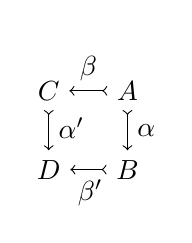
\begin{tikzpicture}
        \node (A) {$A$};
        \node [below of=A] (B) {$B$}; 
        \node [left of=A] (C) {$C$}; 
        \node [left of=B] (D) {$D$}; 
        \begin{scope}[nodes=rectangle]          
        \draw [>->] (A) to node [right,label,pos=0.5] {$\alpha$} (B);
        \draw [>->] (A) to node [above,label,pos=0.5] {$\beta$} (C);
        \draw [>->] (B) to node [below,label,pos=0.45] {$\beta'$} (D); 
        \draw [>->] (C) to node [right,label,pos=0.45] {$\alpha'$} (D);
        \end{scope}
    \end{tikzpicture}
\end{minipage}
\end*{}
\begin{proof}
    \label{subgraph_counting:proof:dcomp_w_u}
%    Since $\operatorname{Mono}(X, B) = \operatorname{Mono}(X, D, \beta')$ by definition of $\operatorname{Mono}(X, B)$ and $\operatorname{Mono}(X, D, \beta')$, the equality $\card{\operatorname{Mono}(X, B)} = \card{\operatorname{Mono}(X, D, \beta')}$ holds.
\begin{claim}
    $\card{\operatorname{Mono}(X, B)} = \card{\operatorname{Mono}(X, D, \beta')}$
\end{claim}
\begin{itemize} 
    \item Inclusion \(\operatorname{Mono}(X, B) \star \beta' \subseteq \operatorname{Mono}(X, D, \beta')\) holds by the definition of $\operatorname{Mono}(X, B)$ and $\operatorname{Mono}(X, D, \beta')$. 
    In fact, if \(\iota  \in \operatorname{Mono}(X, B) \star \beta' \), then there is a monomorphism \(\zeta : X \rightarrowtail B\) satisfying \(\iota = \zeta \star \beta'\). Since $\zeta \star \beta'$ is also a monomorphism\todo{monicity of $\beta'$}, \(\iota\) is also an element of \(\operatorname{Mono}(X, D, \beta')\).
    \item Inclusion \(\operatorname{Mono}(X, B) \star \beta' \supseteq \operatorname{Mono}(X, D, \beta')\) holds by the definition of $\operatorname{Mono}(X, B)$ and $\operatorname{Mono}(X, D, \beta')$.
    Suppose \(\iota \in \operatorname{Mono}(X, D, \beta')\). There is a monomorphism \(\zeta : X \rightarrowtail B\) satisfying \(\iota = \zeta \star \beta'\). It follows that \(\iota = \zeta \star \beta' \in \operatorname{Mono}(X, B) \star \beta'\).
    \item Hence, we have \(\operatorname{Mono}(X, B) \star \beta' = \operatorname{Mono}(X, D, \beta')\).
    \item $\card{\operatorname{Mono}(X, B)} \leq \card{\operatorname{Mono}(X, D, \beta')}$ follows by the injectivity of $\beta'$\todo{monicity of $\beta'$}.
\end{itemize}
\begin{claim}
     $\card{\operatorname{Mono}(X, C, \lnot \beta)} = \card{\operatorname{Mono}(X, D, \lnot \beta', \alpha')}$
   \end{claim}
    \begin{itemize}
        % \item The inclusion \(\operatorname{Mono}(X, C, \lnot \beta) \star \alpha'  \subseteq \operatorname{Mono}(X, D, \lnot \beta', \alpha')\) can be justified as follows. Suppose that \(\iota : X \to D\) is an element of \(\operatorname{Mono}(X, C, \lnot \beta) \star \alpha'\). According to the definition of \(\operatorname{Mono}(X, C, \lnot \beta) \star \alpha'\), there exists \(\eta : X \to C\) in \(\operatorname{Mono}(X, C, \lnot \beta)\) such that \(\iota = \eta \star \alpha'\). We need to show that no \(\zeta : X \to B\) exists such that \(\iota = \zeta \star \beta'\). Assuming the contrary, that such a \(\zeta\) exists. Under this assumption, the following commutative diagram holds:
        \item The inclusion \(\operatorname{Mono}(X, C, \lnot \beta) \star \alpha'  \subseteq \operatorname{Mono}(X, D, \lnot \beta', \alpha')\) can be justified as follows: Suppose \(
            \eta \star \alpha' \in \operatorname{Mono}(X, C, \lnot \beta) \star \alpha'\).
        %  By the definition of \(\operatorname{Mono}(X, C, \lnot \beta) \star \alpha'\), there exists a morphism \(\eta : X \to C\) in \(\operatorname{Mono}(X, C, \lnot \beta)\) such that \(\iota = \). 
         Since $\eta \star \alpha'$ is a monomorphism\todo{monicity of $\alpha'$}, it suffices to show that there is no \(\zeta : X \rightarrowtail B\) such that \(\eta \star \alpha' = \zeta \star \beta'\). Suppose, by contradiction, that such a \(\zeta\) exists, then the following commutative diagram holds:
        \begin{center}
            \begin{tikzpicture}[node distance=10mm]
                \node (A) {A}; 
                \node (B) [above right=of A] {B};
                \node (X) [left = of A] {X};
                \node (D) [below right=of B] {D};
                \node (C) [below right=of A] {C};
                \draw[>->] (A) to node[pos=.7, below] {$\alpha$} (B) ;
                \draw[>->] (C) to  node[pos=0.7, below] {$\alpha'$} (D);
                \draw[>->] (A) -- (C) node[pos=.4, right] {$\beta$};
                \draw[>->] (B) -- (D) node[pos=.4, right] {$\beta'$};
                \draw[>->] (X) -- node[above] {$\zeta$} (B);
                \draw[>->] (X) -- node[below] {$\eta$} (C);
            \end{tikzpicture}
        \end{center} 
        The pushout square \(\square ABDC\) is also a pullback square, by~\autoref{prop:pb_eq_po}. The universal property of the pullback provides a morphism \(\gamma : X \rightarrow A\) such that \(\eta = \gamma \star \beta\). \(\gamma\) is a monomorphism, because \(\eta = \gamma \star \beta\) and $\eta$ is a monomorphism. Therefore, the existence of $\gamma$ contradicts the assumption that \(\eta \in \operatorname{Mono}(X, C, \lnot \beta)\). Thus, \(\iota\) is also an element of \(\operatorname{Mono}(X, D, \lnot \beta', \alpha')\). 
        \item The inclusion \(\operatorname{Mono}(X, C, \lnot \beta) \star \alpha'  \supseteq \operatorname{Mono}(X, D, \lnot \beta', \alpha')\) can be justified as follows. Suppose that \(\iota : X \rightarrowtail D\) is an element of \(\operatorname{Mono}(X, D, \lnot \beta', \alpha')\). According to the definition of \(\operatorname{Mono}(X, D, \lnot \beta', \alpha')\), there exists \(\eta : X \rightarrowtail C\) making 
            \begin{flalign}
                \iota = \eta \star \alpha' \label{eq:etastaralphap}
            \end{flalign}
        We show that \(\eta\) is an element of 
        \(\operatorname{Mono}(X, C, \lnot \beta)\) by contradiction.
        
        Suppose that there is a monomorphism \(\zeta : X \rightarrowtail A\) such that 
        \begin{flalign}
            \eta = \zeta \star \beta \label{eq:zetastarbeta}
        \end{flalign}
        and observe:
        \begin{flalign*}
           \hspace{2cm} \iota &\overset{\operatorname{def}}{=} \eta \star \alpha' &\text{by \eqref{eq:etastaralphap}} 
           \\
                  &\overset{\operatorname{def}}{=} (\zeta \star \beta) \star \alpha' & \text{by \eqref{eq:zetastarbeta}}
                  \\
                  &= \zeta \star (\beta \star \alpha') & \text{by associativity} 
                  \\
                  &= \zeta \star (\alpha \star \beta') &\text{by commutativity of $ABDC$}\\
                  &= (\zeta \star \alpha) \star \beta'
        \end{flalign*}
          There is a contradiction because no such factorization of \(\iota\) should exist as \(\iota \in \operatorname{Mono}(X, D, \lnot \beta', \alpha')\).
        %    Therefore, there is no \(\zeta : X \rightarrow A\) such that \(\eta = \zeta \star \beta\), confirming \(\eta\) as an element of \(\operatorname{Mono}(X, C, \lnot \beta)\). Consequently, \(\iota = \eta \star \alpha'\) is an element of \(\operatorname{Mono}(X, C, \lnot \beta) \star \alpha'\).
        \item We conclude by the monicity of \(\alpha'\). \todo{monicity of $\alpha'$}
        % From \(\operatorname{Mono}(X, C, \lnot \beta) \star \alpha'  \subseteq \operatorname{Mono}(X, D, \lnot \beta', \alpha')\) and \(\operatorname{Mono}(X, C, \lnot \beta) \star \alpha'  \supseteq \operatorname{Mono}(X, D, \lnot \beta', \alpha')\), we conclude \(\operatorname{Mono}(X, C, \lnot \beta) \star \alpha' = \operatorname{Mono}(X, D, \lnot \beta', \alpha')\) and \(\card{\operatorname{Mono}(X, C, \lnot \beta) \star \alpha'} = \card{\operatorname{Mono}(X, D, \lnot \beta', \alpha')}\).
        % Since \(\alpha'\) is monic, \(\card{\operatorname{Mono}(X, C, \lnot \beta)} = \card{\operatorname{Mono}(X, C, \lnot \beta) \star \alpha'}\). Therefore, \(\card{\operatorname{Mono}(X, C, \lnot \beta)} = \card{\operatorname{Mono}(X, D, \lnot \beta', \alpha')}\).
    \end{itemize}
\end{proof} 



\noindent
\begin*{\textbf{\autoref{subgraph_counting:lem:xlnlmxrnr}}}
Let $X$ be a graph. Let $L \overset{l}{\leftarrow} K \overset{r}{\rightarrow} R$ be an injective DPO graph rewriting rule. We have 
\[
   \card{\operatorname{Mono}(X, L, \lnot l)}  - \card{\operatorname{Mono}(X, R, \lnot r)} 
   = 
   \card{\operatorname{Mono}(X, L)}  - \card{\operatorname{Mono}(X, R)} 
    \]
\end*{}
\begin{proof}
    \label{subgraph_counting:proof:lem:xlnlmxrnr}
    \begin{claim}
       $\card{\operatorname{Mono}(X, L, l)} = \card{\operatorname{Mono}(X, R, r)}$
    \end{claim}
    \begin{itemize}
        \item We prove $\card{\operatorname{Mono}(X, L, l)} \leq \card{\operatorname{Mono}(X, R, r)}$ by constructing an injection from $\operatorname{Mono}(X, L, l)$ to $\operatorname{Mono}(X, R, r)$. Let $h \in \operatorname{Mono}(X, L, l)$. By definition, we have $h = g \star l$ for some $g: X \rightarrowtail K$. Thus, $g \star r \in \operatorname{Mono}(X, L, r)$. Let $h' \in \operatorname{Mono}(X, L, l)$ such that $h \neq h'$. We have $h' = g' \star l$ for some $g':X \rightarrowtail K$. We have $g \neq g'$ because otherwise we would have $h = g \star l = g' \star l = h'$. From the monicity of $r$, we conclude $g \star r \neq g' \star r$.
        \item Analoguously, we can prove $\card{\operatorname{Mono}(X, L, l)} \geq \card{\operatorname{Mono}(X, R, r)}$ by constructing an injection from $\operatorname{Mono}(X, R, r)$ to $\operatorname{Mono}(X, L, l)$.
        %  Let $h \in \operatorname{Mono}(X, R, r)$. By definition, we have $h = g \star r$ for some $g: X \rightarrowtail K$. Thus, $g \star l \in \operatorname{Mono}(X, L, l)$.
        % Let $h' \in \operatorname{Mono}(X, R, r)$ such that $h \neq h'$. We have $h' = g' \star l$ for some $g':X \rightarrowtail K$. Since $r$ is monic, we deduce $g \neq g'$. From the monicity of $l$, we conclude $g \star r \neq g' \star r$.
    \end{itemize}


    % we have \[\card{\operatorname{Mono}(X, L, l)} - \card{\operatorname{Mono}(X, R, r)} = 0 \] becase 
    
    Hence, the following equality holds
    \begin{flalign*}
         &\card{\operatorname{Mono}(X, L, \lnot l)}  - \card{\operatorname{Mono}(X, R, \lnot r)}\\
        =&\card{\operatorname{Mono}(X, L) \setminus \operatorname{Mono}(X, L, l)}  - 
            \card{\operatorname{Mono}(X, R) \setminus \operatorname{Mono}(X, R, r)}\\
        =&(\card{\operatorname{Mono}(X, L)} - \card{\operatorname{Mono}(X, L, l)}) - (\card{\operatorname{Mono}(X, R)} - \card{\operatorname{Mono}(X, R, r)}) \\
        =&(\card{\operatorname{Mono}(X, L)} - \card{\operatorname{Mono}(X, R)})
         - (\card{\operatorname{Mono}(X, L, l)} - \card{\operatorname{Mono}(X, R, r)})\\
        = &\card{\operatorname{Mono}(X, L)} - \card{\operatorname{Mono}(X, R)}
    \end{flalign*}
\end{proof}

\noindent
\begin*{\textbf{\autoref{subgraph_counting:lem:w_u_l_not_geq_r_not}}}
\ \newline 
    \noindent 
    \begin{minipage}{0.7\textwidth}
        Let $X$ be a ruler-graph and $\rho = (L \overset{l}{\leftarrowtail} K \overset{r}{\rightarrowtail} R)$ an injective DPO rewriting rule.
        Suppose that $\rho$ is $X$-non-increasing. For every rewriting step induced by the DPO diagram (shown on the right), we have 
        \[
            |\operatorname{Mono}(X, G, \lnot m, \lnot l')| \geq |\operatorname{Mono}(X, H, \lnot m', \lnot r')|
        \]
    \end{minipage}
    \hfill
    \begin{minipage}{0.29\textwidth}
        \hfill
        \resizebox{0.9\textwidth}{!}{
                \begin{tikzpicture}
            \node (k) at (0,1) {K};
            \node (l) at (-2,1) {L};
            \node (r) at (2,1) {R};
            \node (c) at (0,-1) {C};
            \node (g) at (-2,-1) {G};
            \node (h) at (2,-1) {H};
            % \node (rb) at (1.5,-0.5) {$R_X$};
            % \node (h') at (1.5,-1.5) {$H'$};
            % \draw[>->]  (rb) -- (h') node [midway,above] {};
            % \draw[>->]  (c) -- (h') node [midway,above] {};
            \draw[<-<]  (l) -- (k) node [midway,below] {$l$};
            \draw[>->]  (k) -- (r) node [midway,below] {$r$};
            \draw[>->] (c) -- (g) node [midway, above] {$l'$};
            \draw[>->] (c) -- (h) node [midway,above] {$r'$};
            \draw[>->] (l) -- (g) node[midway, right] {$m$};
            \draw[>->] (r) -- (h) node[midway, left] {$m'$};
            \draw[>->] (k) -- (c) node[midway, left] {};
            \node () [at=($(l)!0.5!(c)$)] {$PO$};
            \node () [at=($(r)!0.5!(c)$)] {$PO$};
            % \draw[>->] (rb) to (r);
            % \draw[->] (rb) to (l);
            % \draw[<-<] (rb) to (k);
        \end{tikzpicture}
        }
    \end{minipage}
\end*{}
\begin{proof}
    \label{proof:lem:w_u_l_not_geq_r_not}
    We are going to show that for two arbitrary distinct monomorphisms $h_{XH}', h_{XH}'' \in \operatorname{Mono}(X, H, \lnot m', \lnot r')$, there are two distinct monomorphisms $h_{XG}', h_{XG}'' \in \operatorname{Mono}(X, G, \lnot m, \lnot l')$.

    Let $h_{XH}'\in \operatorname{Mono}(X, H, \lnot m', \lnot r')$ be a monomorphism. In the category \textbf{Graph}, we can construct the following commutative diagram
    \begin{center}
        \resizebox{6cm}{!}{
            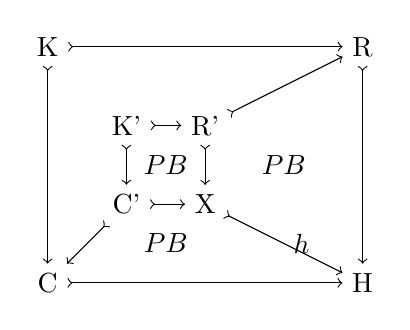
\begin{tikzpicture}
                \node (k) at (0,0) {K};
                \node (r) at (4,0) {R};
                \node (c) at (0,-3) {C};
                \node (h) at (4,-3) {H};
                % \node (rb) at ($\scl*(1.5,-0.5)$) {$R_X$};
                
                % \node (h') at ($\scl*(1.5,-1.5)$) {$H'$};
                % \draw[>->]  (rb) -- (h') node [midway,above] {};
                % \draw[>->]  (c) -- (h') node [midway,above] {};
    
                \draw[<-<]  (r) -- (k) node [midway,above] {};
                \draw[>->] (c) -- (h) node [midway, below] {};
                \draw[>->] (r) -- (h) node[midway, left] {};
                \draw[>->] (k) -- (c) node[midway, left] {};
    
                % \draw[->] (rb) to (l);
                % \draw[<-<] (rb) to (k);
            
                \node (k') at (1,-1) {K'};
                \node (r') at (2,-1) {R'};
                \node (c') at (1,-2) {C'};
                \node () at (1.5,-1.5) {$PB$};
                \node () at (3,-1.5) {$PB$};
                \node () at (1.5,-2.5) {$PB$};
                \node (x) at (2,-2) {X};
                % \draw [->] (x) -- (h') node[midway] {!};
                \draw [>->] (c') -- (x);
                \draw [>->] (r') -- (x);
                \draw [>->] (k') -- (r');
                \draw [>->] (k') -- (c');
                \draw [>->] (c') -- (c);
                % \draw [->] (r') -- (rb);
                % \draw [->] (r') -- (rb);
                % \draw [->] (h') -- (h);
    
                \draw[>->] (r') -- (r);
                \draw[>->] (x) -- (h) node[midway,right] {$h$};
                % \node (rb) at ($\scl*(\sclx*1.5,-0.5)$) {$R_X$};
                % \node (h') at ($\scl*(\sclx*1.5,-1.2)$) {$H'$};
                % \draw[>->]  (rb) -- (h') node [midway,above] {};
                % \draw[>->]  (c) -- (h') node [midway,above] {};
                % \draw[>->]  (rb) -- (h') node [midway,above] {};
                % \draw[>->] (rb) to (r);
                % \draw[<-<] (rb) to (k);
            \end{tikzpicture}
        }
        \end{center} 
    
    $KCHR$ is also pullback, by~\autoref{prop:pb_eq_po}, because it is pushout. 
    Therefore, since $KCHR$ is also pullback and \(
        h_{K'C'} \star h_{C'C} \star h_{CH} =h_{K'R'} \star h_{R'R} \star h_{R'R}
    \) holds, there exists $h_{K'K}:K' \rightarrowtail K$ such that 
    \begin{flalign}
        h_{K'C'} \star h_{C'C} &= h_{K'K} \star h_{KC} \label{kpcpcpckpkkc}
        \\
        h_{K'R'} \star h_{R'R} &= h_{K'K} \star h_{KR} \label{kprprprkpk}
    \end{flalign} 
    
    The square $K'KCC'$ and $K'R'RK$ are pullbacks, by~\autoref{kpcpck_pullback}. Hence, the following commutative diagram holds
    \begin{center}
        \resizebox{6cm}{!}{
            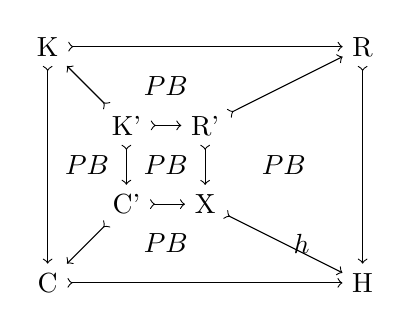
\begin{tikzpicture}
                \node (k) at (0,0) {K};
                \node (r) at (4,0) {R};
                \node (c) at (0,-3) {C};
                \node (h) at (4,-3) {H};
                % \node (rb) at ($\scl*(1.5,-0.5)$) {$R_X$};
                % \node (h') at ($\scl*(1.5,-1.5)$) {$H'$};
                % \draw[>->]  (rb) -- (h') node [midway,above] {};
                % \draw[>->]  (c) -- (h') node [midway,above] {};
                \draw[<-<]  (r) -- (k) node [midway,above] {};
                \draw[>->] (c) -- (h) node [midway, below] {};
                \draw[>->] (r) -- (h) node[midway, left] {};
                \draw[>->] (k) -- (c) node[midway, left] {};
                % \draw[->] (rb) to (l);
                % \draw[<-<] (rb) to (k);
                \node (k') at (1,-1) {K'};
                \node (r') at (2,-1) {R'};
                \node (c') at (1,-2) {C'};
                \node () at (1.5,-1.5) {$PB$};
                \node () at (3,-1.5) {$PB$};
                \node () at (1.5,-2.5) {$PB$};
                \node () at (1.5,-0.5) {$PB$};
                \node () at (0.5,-1.5) {$PB$};
                \node (x) at (2,-2) {X};
                % \draw [->] (x) -- (h') node[midway] {!};
                \draw [>->] (c') -- (x);
                \draw [>->] (r') -- (x);
                \draw [>->] (k') -- (r');
                \draw [>->] (k') -- (c');
                \draw [>->] (c') -- (c);
                % \draw [->] (r') -- (rb);
                % \draw [->] (r') -- (rb);
                % \draw [->] (h') -- (h);
                \draw[>->] (r') -- (r);
                \draw[>->] (x) -- (h) node[midway,right] {$h$};
                % \node (rb) at ($\scl*(\sclx*1.5,-0.5)$) {$R_X$};
                % \node (h') at ($\scl*(\sclx*1.5,-1.2)$) {$H'$};
                % \draw[>->]  (rb) -- (h') node [midway,above] {};
                % \draw[>->]  (c) -- (h') node [midway,above] {};
                % \draw[>->]  (rb) -- (h') node [midway,above] {};
                % \draw[>->] (rb) to (r);
                % \draw[<-<] (rb) to (k);
                \draw[>->] (k') -- (k) ;
            \end{tikzpicture}
        }
        \end{center} 

    \todo{use: assumption: non increasing}
    Since the rule is by assumption $X$-non-increasing, there is a morphism $h_{R'L}$ such that $K'KLR'$ is commutative.
    
    $K'C'XR'$ is a pushout by~\autoref{kpcpxrp_po}. 
    
    Thus, the following commutative diagram holds
    \begin{center}
        \resizebox{6cm}{!}{
            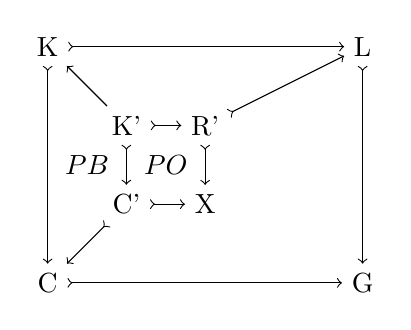
\begin{tikzpicture}
                \node (k) at (0,0) {K};
                \node (r) at (4,0) {L};
                \node (c) at (0,-3) {C};
                \node (h) at (4,-3) {G};
                % \node (rb) at ($\scl*(1.5,-0.5)$) {$R_X$};
                
                % \node (h') at ($\scl*(1.5,-1.5)$) {$H'$};
                % \draw[>->]  (rb) -- (h') node [midway,above] {};
                % \draw[>->]  (c) -- (h') node [midway,above] {};
    
                \draw[<-<]  (r) -- (k) node [midway,above] {};
                \draw[>->] (c) -- (h) node [midway, below] {};
                \draw[>->] (r) -- (h) node[midway, left] {};
                \draw[>->] (k) -- (c) node[midway, left] {};
    
                % \draw[->] (rb) to (l);
                % \draw[<-<] (rb) to (k);
            
                \node (k') at (1,-1) {K'};
                \node (r') at (2,-1) {R'};
                \node (c') at (1,-2) {C'};
                \node () at (1.5,-1.5) {$PO$};
                % \node () at (1.5,-0.5) {$PB$};
                \node () at (0.5,-1.5) {$PB$};
                % \node () at (3,-1.5) {$PB$};
                % \node () at (1.5,-2.5) {$PB$};
                \node (x) at (2,-2) {X};
                % \draw [->] (x) -- (h') node[midway] {!};
                \draw [>->] (c') -- (x);
                \draw [>->] (r') -- (x);
                \draw [>->] (k') -- (r');
                \draw [>->] (k') -- (c');
                \draw [>->] (c') -- (c);
                \draw [->] (k') -- (k);
                % \draw [->] (r') -- (rb);
                % \draw [->] (r') -- (rb);
                % \draw [->] (h') -- (h);
    
                \draw[>->] (r') -- (r);
                % \draw[>->] (x) -- (h) node[midway,right] {$h$};
                % \node (rb) at ($\scl*(\sclx*1.5,-0.5)$) {$R_X$};
                % \node (h') at ($\scl*(\sclx*1.5,-1.2)$) {$H'$};
                % \draw[>->]  (rb) -- (h') node [midway,above] {};
                % \draw[>->]  (c) -- (h') node [midway,above] {};
                % \draw[>->]  (rb) -- (h') node [midway,above] {};
                % \draw[>->] (rb) to (r);
                % \draw[<-<] (rb) to (k);
            \end{tikzpicture}
        }
        \end{center} 

    By~\autoref{lem:g_monic}, there is a unique monomorphism $h_{XG}':X \rightarrowtail G$ such that $h_{C'X} \star h_{XG}' = h_{C'C} \star h_{CG}$ and $h_{R'X} \star h_{XG}' = h_{R'L} \star h_{LG}$.

    The monomorphism $h_{XG}'$ is in the set $\operatorname{Mono}(X, G, \lnot m, \lnot l')$, by $h_{XH}'\in \operatorname{Mono}(X, H, \lnot m', \lnot r')$ and~\autoref{subgraph_counting:def:creates_more_x_on_the_left}. 
    Intuitively, $h_{XH}'\in \operatorname{Mono}(X, H, \lnot m', \lnot r')$ implies that some elements in $X$ are mapped onto $h_{RH}(R) \setminus (r \star h_{RH})(K)$. By the first assumption of~\autoref{subgraph_counting:def:creates_more_x_on_the_left}, these elements are mapped onto $h_{LG}(L) \setminus (l \star h_{LG})(K)$.

    
    The monomorphism \( h_{XG}' \) belongs to the set \( \operatorname{Mono}(X, G, \lnot m, \lnot l') \), due to \( h_{XH}' \in \operatorname{Mono}(X, H, \lnot m', \lnot r') \) and~\autoref{subgraph_counting:def:creates_more_x_on_the_left}. Intuitively, \( h_{XH}' \in \operatorname{Mono}(X, H, \lnot m', \lnot r') \) implies that certain elements of \( X \) are mapped into \( h_{RH}(R) \setminus (r \star h_{RH})(K) \). By the second assumption of~\autoref{subgraph_counting:def:creates_more_x_on_the_left}, these elements are also mapped into \( h_{LG}(L) \setminus (l \star h_{LG})(K) \).

     \todo{use; def non-increase; condition 1}
    
    \todo{todo to do : detailler}

    Let $h_{XH}'':X \rightarrowtail H$ be a monomorphism such that 
    \begin{flalign}
        h_{XH}' \neq h_{XH}'' \label{hpneqh}
    \end{flalign}
    
    In the category \textbf{Graph}, we can construct the following commutative diagram:
    \begin{center}
        \resizebox{6cm}{!}{
            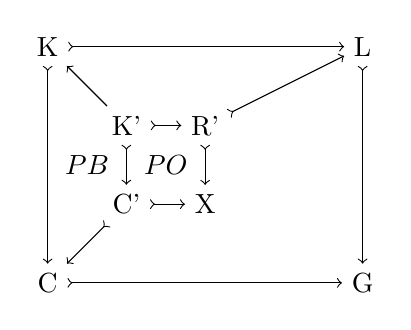
\begin{tikzpicture}
                \node (k) at (0,0) {K};
                \node (r) at (4,0) {L};
                \node (c) at (0,-3) {C};
                \node (h) at (4,-3) {G};
                % \node (rb) at ($\scl*(1.5,-0.5)$) {$R_X$};
                
                % \node (h') at ($\scl*(1.5,-1.5)$) {$H'$};
                % \draw[>->]  (rb) -- (h') node [midway,above] {};
                % \draw[>->]  (c) -- (h') node [midway,above] {};
    
                \draw[<-<]  (r) -- (k) node [midway,above] {};
                \draw[>->] (c) -- (h) node [midway, below] {};
                \draw[>->] (r) -- (h) node[midway, left] {};
                \draw[>->] (k) -- (c) node[midway, left] {};
    
                % \draw[->] (rb) to (l);
                % \draw[<-<] (rb) to (k);
            
                \node (k') at (1,-1) {K'};
                \node (r') at (2,-1) {R'};
                \node (c') at (1,-2) {C'};
                \node () at (1.5,-1.5) {$PO$};
                % \node () at (1.5,-0.5) {$PB$};
                \node () at (0.5,-1.5) {$PB$};
                % \node () at (3,-1.5) {$PB$};
                % \node () at (1.5,-2.5) {$PB$};
                \node (x) at (2,-2) {X};
                % \draw [->] (x) -- (h') node[midway] {!};
                \draw [>->] (c') -- (x);
                \draw [>->] (r') -- (x);
                \draw [>->] (k') -- (r');
                \draw [>->] (k') -- (c');
                \draw [>->] (c') -- (c);
                \draw [->] (k') -- (k);
                % \draw [->] (r') -- (rb);
                % \draw [->] (r') -- (rb);
                % \draw [->] (h') -- (h);
    
                \draw[>->] (r') -- (r);
                % \draw[>->] (x) -- (h) node[midway,right] {$h$};
                % \node (rb) at ($\scl*(\sclx*1.5,-0.5)$) {$R_X$};
                % \node (h') at ($\scl*(\sclx*1.5,-1.2)$) {$H'$};
                % \draw[>->]  (rb) -- (h') node [midway,above] {};
                % \draw[>->]  (c) -- (h') node [midway,above] {};
                % \draw[>->]  (rb) -- (h') node [midway,above] {};
                % \draw[>->] (rb) to (r);
                % \draw[<-<] (rb) to (k);
            \end{tikzpicture}
        }
        \end{center} 

    Analoguously, there exists a unique monomorphism $h_{XG}'':X \rightarrowtail G$ such that $h_{C''X} \star h_{XG} ''= h_{C''C} \star h_{CG}$ and $h_{R''X} \star h_{XG}'' = h_{R''L} \star h_{LG}$.
    
    By \eqref{hpneqh} and~\autoref{lem:h_hp_diff_g_gp_diff}, we have $h_{XG} \neq h_{XG}'$.
\end{proof}



\noindent
\begin*{\textbf{\autoref{subgraph_counting:lem:w_g_geq_w_h_leq}}}[Decreasing step]
Let $\rho = (L \overset{l}{\leftarrowtail} K \overset{r}{\rightarrowtail} R)$ be an injective DPO rewriting rule,
\( \mathbb{X} \) a set of ruler-graphs,
\( s_{\mathbb{X}} \colon \mathbb{X} \to \mathbb{N} \) a weight function,
and \( G \Rightarrow_{\rho,\mathfrak{M}} H \) a rewriting step. 
If $\rho$ is \( X \)-non-increasing for every ruler-graph \( X \in \mathbb{X} \), then:\[
    w_{s_\mathbb{X}}(G) - w_{s_\mathbb{X}}(H) 
    \geq 
    w_{s_\mathbb{X}}(L) - w_{s_\mathbb{X}}(R)
\]
\end*{}
\begin{proof}
    \label{subgraph_counting:proof:lem:w_g_geq_w_h_leq}
    Let the following diagram be the witness diagram of the rewriting step
    \begin{center}
        \begin{tikzpicture}
            \node (k) at (0,1) {K};
            \node (l) at (-2,1) {L};
            \node (r) at (2,1) {R};
            \node (c) at (0,-1) {C};
            \node (g) at (-2,-1) {G};
            \node (h) at (2,-1) {H};
            \draw[<-<]  (l) -- (k) node [midway,below] {$l$};
            \draw[>->]  (k) -- (r) node [midway,below] {$r$};
            \draw[>->] (c) -- (g) node [midway, above] {$l'$};
            \draw[>->] (c) -- (h) node [midway,above] {$r'$};
            \draw[>->] (l) -- (g) node[midway, right] {$m$};
            \draw[>->] (r) -- (h) node[midway, left] {$m'$};
            \draw[>->] (k) -- (c) node[midway, left] {};
            \node () [at=($(l)!0.5!(c)$)] {$PO$};
            \node () [at=($(r)!0.5!(c)$)] {$PO$};
        \end{tikzpicture}
    \end{center}
    Let $X \in \mathbb{X}$.

    We have 
    \begin{flalign*}
        & \card{\operatorname{Mono}(X,G)}
            % \overset{\operatorname{def}}{=} 
            % w_{T_\Sigma}(t_G) 
        \\
        % =& \Psi_{G}\\
        =& 
        \card{\operatorname{Mono}(X,G,l')
        \uplus
         \operatorname{Mono}(X,G,\lnot l',m)
        \uplus
         \operatorname{Mono}(X,G,\lnot l',\lnot m)}\\
        =& 
        \card{\operatorname{Mono}(X,G,l')}
        +
         \card{\operatorname{Mono}(X,G,\lnot l',m)}
        +
        \card{\operatorname{Mono}(X,G,\lnot l',\lnot m)}
        \\
    =& \card{\operatorname{Mono}(X,C)}
            +
            \card{\operatorname{Mono}(X, L, \lnot l)} 
            +
            \card{\operatorname{Mono}(X, G,\lnot l', \lnot m)} 
        &  \text{by~\autoref{subgraph_counting:lem:decomp_w_u}}
    \end{flalign*}
    and
    \begin{flalign*}
        % ligne 1
        &\card{\operatorname{Mono}(X,H)}
        % \overset{\operatorname{def}}{=}  
        %     w_{T_\Sigma}(t_H )
        \\
        =& 
        \card{\operatorname{Mono}(X,H,r')
        \uplus
            \operatorname{Mono}(X,H,\lnot r',m')
        \uplus
            \operatorname{Mono}(X,H,\lnot r',\lnot m')}
        \\
        =& 
        \card{\operatorname{Mono}(X,H,r')}
        +
         \card{\operatorname{Mono}(X,H,\lnot r',m')}
        +
        \card{\operatorname{Mono}(X,H,\lnot r',\lnot m')}
        \\
        % = & \Psi_{H} \\
        % ligne 2
        = &
            \card{\operatorname{Mono}(X,C)}
            +
            \card{\operatorname{Mono}(X, R, \lnot r)} 
            +
            \card{\operatorname{Mono}(X, H, \lnot r', \lnot m')}
        % ( 
        %             w_{T_\Sigma} (h_{RH} \star t_H ) + w_{T_\Sigma} (h_{CH} \star t_H  -h_{KC}) 
        % )
        %         +  w_{T_\Sigma}(t_H  - \{h_{RH},h_{CH} \})  
        &  \text{by~\autoref{subgraph_counting:lem:decomp_w_u}}
    \end{flalign*}
    Therefore, the following inequality holds
     \begin{flalign*}
           &\card{\operatorname{Mono}(X,G)} - \card{\operatorname{Mono}(X,H)} &\\
           =&(\card{\operatorname{Mono}(X, L, \lnot l)} - \card{\operatorname{Mono}(X, R, \lnot r)}) + 
            (\card{\operatorname{Mono}(X, G, \lnot l', \lnot m)} - \card{\operatorname{Mono}(X, H, \lnot r', \lnot m')}) \\
       \geq& \card{\operatorname{Mono}(X, L, \lnot l)} - \card{\operatorname{Mono}(X, R, \lnot r)} \hspace{3cm} 
       \text{by~\autoref{subgraph_counting:lem:w_u_l_not_geq_r_not}} \\
          =& \card{\operatorname{Mono}(X, L)} - \card{\operatorname{Mono}(X, R)} \hspace{3cm} 
          \text{by~\autoref{subgraph_counting:lem:xlnlmxrnr}}
     \end{flalign*}
     Thus, the following inequality holds
     \begin{flalign*}
          &w_{s_\mathbb{X}}(G) - w_{s_\mathbb{X}}(H)
          \\
         =&\sum_{X \in \mathbb{X}}^{}w(X) * |\operatorname{Mono}(X,G)| - \sum_{X \in \mathbb{X}}^{}w(X) * |\operatorname{Mono}(X,H)|
         \\
         =&\sum_{X \in \mathbb{X}}^{}w(X) * \left( \card{\operatorname{Mono}(X,G)} -  \card{\operatorname{Mono}(X,H)} \right)
         \\
         \geq&\sum_{X \in \mathbb{X}}^{}w(X) * \left(  \card{\operatorname{Mono}(X,L)}- \card{\operatorname{Mono}(X,R)} \right)
         \\
         = &\sum_{X \in \mathbb{X}}^{}w(X) * \card{\operatorname{Mono}(X,L)} -  \sum_{X \in \mathbb{X}}^{}w(X) * \card{\operatorname{Mono}(X,R)} 
         \\
         = & w_{s_\mathbb{X}}(L) - w_{s_\mathbb{X}}(R)
     \end{flalign*}
    \qed
\end{proof}

\noindent
\begin*{\textbf{\autoref{subgraph_counting:thm:termination_grs}}}[Termination]
    Let \(\mathcal{A}\) and \(\mathcal{B}\) be sets of injective DPO rewriting rules, $\mathbb{X}$ a set of ruler-graphs and $s_\mathbb{X}$ a weight function. If the following hold
    \begin{enumerate}
        \item\label{subgraph_counting:thm:termination_grs:assump:1} $\rho$ is $X$-non-increasing for every rule $\rho \in \mathcal{A} \cup \mathcal{B}$ and for every ruler-graph $X \in \mathbb{X}$,
        \item\label{thm:termination_grs:assump:2} \( w_{s_\mathbb{X}}(lhs(\rho)) > w_{s_\mathbb{X}}(rhs(\rho)) \) for every rule \(\rho \in \mathcal{A}\),
        \item\label{thm:termination_grs:assump:3} \( w_{s_\mathbb{X}}(lhs(\rho)) \geq w_{s_\mathbb{X}}(rhs(\rho)) \) for every rule \(\rho \in \mathcal{B}\).
    \end{enumerate}
    Then \(\Rightarrow_{\mathcal{A},\mathcal{M}}\) terminates relative to \(\Rightarrow_{\mathcal{B},\mathcal{M}}\).
\end*{}
\begin{proof}
    \label{subgraph_counting:proof:thm:termination_grs}
    
    By assumption \eqref{subgraph_counting:thm:termination_grs:assump:1} and ~\autoref{subgraph_counting:lem:w_g_geq_w_h_leq}, the inequality \(
        w_{s_\mathbb{X}}(G) - w_{s_\mathbb{X}}(H) 
        \geq 
        w_{s_\mathbb{X}}(\operatorname{lhs}(\rho)) - w_{s_\mathbb{X}}(\operatorname{rhs}(\rho))
    \) holds for all rules $\rho \in \mathcal{A} \cup \mathcal{B}$ and for all rewriting steps $G \Rightarrow_{\rho, \mathcal{M}} H$.
    
    \noindent From assumptions \eqref{thm:termination_grs:assump:2} and \eqref{thm:termination_grs:assump:3}, we deduce 
    \begin{itemize}
        \item \( w_{s_\mathbb{X}}(G) > w_{s_\mathbb{X}}(H) \) for every rule \(\rho \in \mathcal{A}\);
        \item  \( w_{s_\mathbb{X}}(G) \geq w_{s_\mathbb{X}}(H) \) for every rule \(\rho \in \mathcal{B}\).
    \end{itemize}
    Since $w_{s_\mathbb{X}}(G) \in \mathbb{N}$ for all graph $G$. Every rewriting chain can only have a finite number of rewriting steps using rules in $\mathcal{A}$.
\end{proof} 